\documentclass[11pt]{article}
\usepackage[utf8]{inputenc}
\usepackage[myheadings]{fullpage}

% Package for headers 
\usepackage{fancyhdr}
\usepackage{lastpage}

% For figures and stuff
\usepackage{graphicx, wrapfig, setspace, booktabs}
\usepackage[T1]{fontenc}
\usepackage{subfigure}

% Change for different font sizes and families
\usepackage[font=small, labelfont=bf]{caption}
\usepackage{fourier}
\usepackage[protrusion=true]{microtype}

% Maths
\usepackage{amsmath,amssymb}
\usepackage{float}
\usepackage{graphicx}
\usepackage{wrapfig}
\usepackage[colorinlistoftodos]{todonotes}
\usepackage[colorlinks=true, allcolors=blue]{hyperref}
\usepackage{mathtools}
\usepackage{mhchem}
\usepackage{tensor}
\usepackage{gensymb}
\usepackage{fancyhdr}
\usepackage{braket}
\usepackage{tikz}
\usetikzlibrary{shapes.geometric, arrows}

\tikzstyle{startstop} = [rectangle, rounded corners, minimum width=3cm, minimum height=1cm, text centered, draw=black, text width = 6cm]
\tikzstyle{arrow} = [thick,->,>=stealth]
\tikzstyle{line} = [thick,-,>=stealth]

% Bibliography
% \usepackage{biblatex} 
% \addbibresource{references.bib}

%% Language and font encodings
\usepackage[english]{babel}


\newcommand{\HRule}[1]{\rule{\linewidth}{#1}}
\onehalfspacing
\setcounter{tocdepth}{5}
\setcounter{secnumdepth}{5}

%% Sets page size and margins
\usepackage[a4paper,top=2cm,bottom=1.5cm,left=2cm,right=2cm,marginparwidth=1.5cm]{geometry}

\pagestyle{fancy}
\fancyhf{}

% Header and footer information
\setlength{\marginparwidth}{2cm}
\setlength\headheight{15pt}
\fancyhead[L]{Review of Quantum Sensor} 
\fancyhead[R]{Jiheng Duan}
\fancyfoot[R]{\thepage}


\begin{document}

\date{}

% Do not change anything here except in \LARGE \textbf{This is the title of the essay} 
% /hline before and after the title makes those horoziontal lines appear, you can change the appearance by changing the 2pt to different sizees
\title{ \normalsize University of Macau
		\\ [1.0cm]
		% Change to your faculty if needed
		
\includegraphics[width=25mm]{figures/1280px-University_of_Macau.svg.png}\\[.5cm]
		Faculty of Science and Technology\\
		\HRule{2pt} \\
		\LARGE \textbf{Quantum Sensor: A brief Overview and Quantum Magnetic Field Sensor} %para que quede encerrado en las lineas
		\HRule{2pt} \\ [0.5cm]
		\normalsize \today \vspace*{5\baselineskip}}
		
\date{}

\author{
		Jiheng Duan  \\
		 DB928205}
		 
\maketitle

%\newpage
\newpage

\section*{Abstract}
% Add your own abstract here
Quantum sensor is a sophisticated research area that actually is a type of physical sensor. This essay will briefly introduce the fundamental concepts of the mechanism of quantum senor and qubit system, including some examples of qubit system setup and a real magnetic field quantum sensor based on diamond nitrogen-vacancy(N-V) center defects qubits. 

\paragraph*{Keywords}: Quantum sensor, qubit, diamond N-V center defect qubit, magnetic field sensor.

% Uncomment the next line if you want keywords/index terms after the abstract. 
%\textit{\textbf{Keywords}: lorem, ipsum, dolor}
\section{Introduction}
As the development of quantum information technology, quantum mechanics had been applied on various research domains such as quantum cryptography, quantum algorithm, quantum processor, superconducting quantum interference devices(SQUID), and so on, in which quantum superposition and quantum interference played a deterministic role. A vast amount of progress was achieved during the quantum mechanics combined with different research subjects such as the quantum processor Sycamore which finish a task for twenty-five million faster than supercomputer\cite{arute2019quantum}, the coherent Ising machine using degenerate optical parametric oscillators to solve combinatorial optimization problems\cite{2016incoherent}, a powerful quantum algorithm analogized from classical simulated annealing algorithm\cite{kirkpatrick1983optimization} called quantum annealing with an experimental setup basing on coupling flux qubit systems\cite{johnson2011quantum}. Simultaneously, with the evolution of semiconducting physics and superconducting effects, the classical physical sensor branch out another feature combining with quantum systems instead of using classical physical systems.

In order to detect and store vast of information of physical quantities, researchers prefer to use the qubit system, based on the superposition principle of qubit ground state $\ket{g}$ and excited state $\ket{e}$. Different from classical digital bit which can only choose 1 or 0 simultaneously, qubit could be 0 and 1 simultaneously which indicates a single qubit will carry more information than a single classical bit. However, quantum systems, compared with classical physical systems, are more susceptible and fragile, as a small perturbation will change the spectrum of an artificial atom system and the quantum decoherence will lose the information of the system. 

Since the discovery of new qubit systems, like superconducting qubit, light polarization qubit, and diamond N-V center qubit, etc., the development of quantum sensors has become prosperous and some experimental schemes became commercial products. The quantum light meter produced by apogee instruments company with high sensitivity can detect the intensity of the light source which can be applied to the evaluation of light pollution. This applied sensor has found commercial market decades before computers which is under the experimental process till now. The other type of qubit, such as diamond N-V defect center\cite{lee2019ion} based and trapped ions\cite{matsuzaki2016hybrid} based magnetic field sensors, are under processing or only contain theoretical experiment design. These concepts will be discussed in the features and difficulties of the quantum sensor part in this essay.
% Bibliography usage
% Whenever you find any source make sure to get the BibTEX citation. Add it to the references.bib file. To cite the reference, use \cite{TitleOfTheReference}

\section{Quantum Sensing}
Quantum sensing is normally used to interpret one of the following concepts\cite{degen2017quantum}:
	\begin{enumerate}
		\item Measuring a classical or quantum physical quantity through a quantum system. The quantum is characterized by several quantized energy levels, usually are two-level systems. The candidate systems are spin qubit system, superconducting qubit system, neutral atoms, artificial atoms, or trapped ions.
		\item Measuring physical quantity based on quantum coherence, like the superposition of quantized states.
		\item Using the concepts and properties of quantum entanglement to improve the sensitivity and precision of the result that is measured by the physical system.
	\end{enumerate}
From the definitions of quantum sensing, vast physical systems are included in the first two enumerations. Although it says the system is "quantum", actually it contains such an amount of "semi-classical" systems which can be recognized as not strictly "quantum". The example of this "semi-classical" system is given by, in optics, a theory called classical entanglement and people  use this phenomena to build up a layout of using degenerate optical oscillators to realize Shor's algorithm\cite{shor1994algorithms}. The third definition, describes the advantages of applying quantum sensing, that is more sensitive and precise than classical physical system's detection. As quantum entanglement mathematically is the tensor product of different Hilbert spaces. During the entangled period, the information of detected system will be kept in the system without decaying out to the environment which is the reason of precise measurement. The high sensitivity is contributed by small perturbation will split out the energy level which gives us, in read out signal point of view, a obvious changes on the magnitude of signal or widths of wave packets. For more information of the detector, quantum sensor, will be introduced in the following section including quantum sensing protocol and qubit system.


\section{Quantum Sensors}
Actually, the quantum sensor is a quantum system with several constraints. Consequently, qubit systems, which will be introduced in the following section, are the first choices with no more candidates. Analogizing to DiVincenzo criteria for quantum computation, our candidates should satisfy some conditions.
	\begin{enumerate}
		\item The energy level of the quantum system should be discrete and solvable by applying current methods in quantum mechanics.
		\item The quantum system should be tunable by applying a time-dependent external field like the electric field, microwave, or magnetic field.
		\item The quantum system should be able to be initialized and the initial state should be exactly known. Additionally, the information of states after time-evolution should be readable in the readout step.
		\item The interaction between the quantum system and exterior physical objects which can contribute a  potential term $\hat{V}(t)$ in system Hamiltonian $\hat{H}(t)$. 
	\end{enumerate}
The first condition gives us the fundamental requirement of the selected system. Especially, we assume it to be a two-level system with a ground state $\ket{0}$ and an excited state $\ket{1}$. The transition between $\ket{0}$ and $\ket{1}$ is given by absorbing(or emitting) energy $E = \hbar \omega_0$ where $\omega_0 $ states the transition frequency. Quantum sensing exploits changes in the transition frequency by coupling the two energy level systems with an external field. An example is the Jaynes-Cummings model, a theoretical model in quantum optics that describes an atom system whose two energy levels interact with a quantized mode of an optical cavity field. By tuning the optical field, the energy level of the artificial atom would split into entangled states and we could rotate and linearly combine basis to form a set of new states called dressed state which could diagonalize the system Hamiltonian. This example also holds for the second condition, which means we could apply microwave to control the transition between particular atom energy level or dressed state. The energy level is solvable means using like, for example, the perturbation theory which could analytically solve the split of energy level and the corrections of new states. 

The initialization of states is necessary. This condition could be understood from the state evolution under Schrödinger's equation where initialization could be viewed as the initial conditions of the differential equation describing the dynamics of the system. Initialization, in superconducting qubits system, usually by cooling down the system to estimate heat-driven effects. The electron inside the superconductors form copper pairs by exchanging phonons are condensed in the lowest energy state which is around Fermi's energy level. So, the initial states of the detecting system could be constructed in this way.

An important characteristic of quantum sensors is their "intrinsic sensitivity"\cite{degen2017quantum}. In another word, quantum sensors are always expected to provide a strong feedback signal compares to the original signal after a slight change in the detected quantity and it should be minimally affected by environmental noise like heat noise. Typically, the sensitivity scale of a quantum sensor can be formulated by\cite{degen2017quantum}
\begin{equation}
	\text{sensitivity} \propto \frac{1}{\gamma\sqrt{T_\chi}}
\end{equation} 
Where $\gamma$ si the above transduction parameter and $T_\chi$ is decoherence time which reflect the capability of system against noises. Decoherence means the quantum system will lose its interference between different states or says the stored information will lose. That actually is the biggest enemy of quantum computing and, by analogizing, quantum sensor. So, researchers nowadays are putting on effort to delay the decoherence time as long as possible to forbid losing information. 

\section{Qubits and Qubit System}
A quantum system containing two energy levels with a ground state $\ket{g}$ and an excited state $\ket{e}$ is called a qubit, see Fig.1 (a) and (b). Analog to classical bits, quantum bits, or just say qubits, has the ability to store information. Especially, qubits could use its superposition principle to generate an infinite number of states which could represent a vast amount of different information in a single qubit system. For example, we could define the readout of superposition state $\ket{\phi} = \alpha_1\ket{g} + \alpha_2\ket{e}$ represents the information "1001" and another state$\ket{\psi} = \beta_1\ket{g} + \beta_2\ket{e}$ represents "0011" etc..  

In order to store such an amount of information, coupling several qubit systems is significant and necessary for building up a scheme of quantum sensors or, more generally, every quantum computer. Mathematically, coupled systems mean the differential equations which predict the evolution of the total system have several mixed quantities terms, or called coupling terms. In classical mechanics, based on Hamilton equations of motion
\begin{equation}
	\dot{q}_i = \frac{\partial H}{\partial p_i}, \ \dot{p}_i = -\frac{\partial H}{\partial q_i}
\end{equation}
where $p_i$ is general momentum and $q_i$ is displacement in $i$th general coordinates. $\dot{q}$ means time derivative $\frac{\partial q}{\partial t}$. It indicates the system Hamiltonian should contain several coupled terms in order to formulate a set of coupled differential equations. A famous example is the Wilberforce pendulum, which is a long suspended spring with a mass attached at the lower end, which is free to rotate around the vertical axis, twisting the spring through a non-linear-coupling\cite{avendano2020closed}. The Hamiltonian of mass $m$ with rotational inertia $I$ under weak coupling is given by 
\begin{equation}
	H = \frac{1}{2m}p_x^2 + \frac{1}{2I} p_y^2 + \frac{1}{2} kx^2 + \frac{1}{2} \kappa y^2 + g x y
\end{equation}
where $x$ direction is parallel to the vertical spring with spring constant $k$ and $y$ stands the horizontal rotational angle. $\kappa$ means torsional constant and $g$ is the coupling strength. We could clearly see the coupled term is formulated by $gxy$. 

This property also holds in quantum mechanics with coupled operators in Hilbert spaces generated from the tensor product of different Hilbert spaces. Actually, from qubit's point of view, two-qubit systems $A$ and $B$ have their Hamiltonian $\hat{H}_A$ and $\hat{H}_B$. The coupled system's Hamiltonian is formulated by tensor product
\begin{equation}
	\hat{H} = \hat{H}_A \bigotimes I + I \bigotimes \hat{H}_B + \hat{H}_{\text{coupling}}
\end{equation}
where $I$ is the identity matrix. As qubit systems are the first choice of the candidates of quantum sensors, they also need some external field input to manipulate the system, or send signals into the system or read out the final results. Therefore, In quantum sensors, actually, qubit system could be also coupled with an external field, like an optical cavity. For the following discussion, we purpose the total Hamiltonian of the quantum sensor system is formulated by a generic Hamiltonian
\begin{equation}
	\hat{H}(t) = \hat{H}_0 + \hat{H}_V(t) + \hat{H}_{\text{control}}(t)
\end{equation}
where $\hat{H}_0$ is the initial Hamiltonian of the coupled system, $\hat{H}_V(t)$ is the Hamiltonian contributed by the input signal that forms a potential term. $\hat{H}_{control}(t)$ performs the manipulation of evolution and parametrization of coupled qubit system before, during, or after the sensing process. In the description of quantum sensing protocol, instead of directly using Hamiltonian applying on the initialized ground state, we use a propagator $\hat{U}_H$ to propagate out initial state into the desired target state $\ket{\psi_0} = \hat{U}_H \ket{0}$. These Protocols will be discussed in the following section.

\begin{figure}
	\centering
	\subfigure[A simple demonstration of two-energy-level quantum system. ]{
		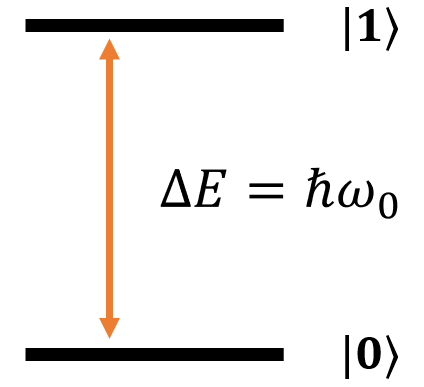
\includegraphics[width=0.25\textwidth]{figures/qubit.png}
	}
	\subfigure[A brief comparision between classical bit and qubit. The qubit part is formulated by Bloch sphare to get a clear visualization of superposition of qubit ground state and excited state and the phase inforation.]{
		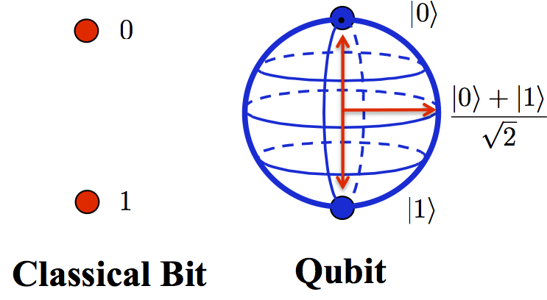
\includegraphics[width=0.45\textwidth]{figures/bloch sphere.png}
	}
	\caption{Qubit demonstration.}
\end{figure}

\section{Quantum Sensing Protocol}

Experiment setup and processing steps of quantum sensing are quite related to a generic sequence of the initialization of sensors, interaction with the input signal, readout of data, and signal estimation. This sequence is shown in flow chart form in Fig.3 in the appendix which could be concluded as a protocol recognized as quantum sensing protocol. This protocol could be summarized as following enumerates\cite{degen2017quantum}:
	\begin{enumerate}
		\item The initialization of state is necessary and the initial basis $\ket{0}$ should be known.
		\item The state of the quantum sensor is transformed into the desired initial sensing state, mainly is a superposition state, $\ket{\psi_0} = \hat{U}_a\ket{0}$ by applying a propagator $\hat{U}_a$, which are usually a set of control pulses, on the initial state $\ket{0}$. 
		\item The quantum sensor system evolves under the Hamiltonian $\hat{H}$[Eq. (4)] for an instantaneous time $t$, described by a propagator $\hat{U}_H = \exp(-\frac{i\hat{H}t}{\hbar})$. After the sensing process is done, at that instantaneous time $t$, the final state of sensor is 
			\begin{equation}
				\ket{\psi(t)} = \hat{U}_H(0,t)\ket{\psi_0} = c_0 \ket{\psi_0} + c_1 \ket{\psi_1}
			\end{equation}
		where $\ket{\psi_1}$ is the state that orthogonal to $\ket{\psi_0}$, and $c_0,c_1$ are complex numbers.
		\item The state of quantum sensor is transformed into the readout state $\ket{\alpha} = \hat{U}_b\ket{\psi(t)} = c'_0\ket{0'} + c'_1\ket{1'}$ by applying a propagator $\hat{U}_b$. It unnecessary to choose you initial state also be your read out state, which mathematically indicates that basis sets satisfy $\{\ket{0'},\ket{1'}\} = \{\ket{0}, \ket{1}\}$ and operators follow $\hat{U}_b = \hat{U}^\dagger_a$, unless you desire to simplify the representations. 
		\item Using each state to take the inner product with the readout state to get the population of the system stay in excited states $\ket{1}$. It could be concluded in the following relation
			\begin{equation}
				p = 1-|c_0|^2 = |c_1|^2
			\end{equation}
		where we define $p = |c_1|^2$ and that actually is the measurable transition probability that the qubit changed its state during time $t$. This result is like a binary answer that is detected by the measurement of apparent physical quantities such as current, number of photons, or the polarization of light. So, indeed to precisely estimate for transition probability $p$, repeated measurements are required.  
		\item By repeating measurement, an average value of transition probability should be reached. In some situations, it is required to record a set of values $\{p_k\}$.
		\item The final result of transition probability $p$ should be time-dependent and Hamiltonian-dependent. It is necessary to generate the desired signal from the recorded data $\{p_k\}$ using a signal producer.
	\end{enumerate}


\section{A Setup of Magnetic Field Quantum Sensor}
A magnetic field quantum sensor based on an electron spin and nuclear spin in nitrogen-vacancy center defect diamond is a theoretical setup by Yuichiro Matsuzaki et al.\cite{matsuzaki2016hybrid} and published in Physical Review A in 2016, aiming to detect weak magnetic field with high precision, accuracy, and sensitivity. The key point of this design is using the long-life nuclear spin as a quantum register to memory the detected information, actually is the accumulated phase difference of pulse, by the electron which has a short decoherence time. The information changes between a spin electron and a spin nuclear are manipulated by a controlled-NOT (C-NOT) gate which has been already demonstrated in \cite{neumann2008multipartite}. Their theoretical setup is shown in Fig.2 (a) with an atomic force microscopy directly touch with nano-scale diamond to read out the stored information in the spin nuclear. C-NOT gate could be realized by injecting microwave into diamond directly. The spin state of the electron is measured by an optical laser based on the absorption spectrum of the electron spin state and a photon detector is introduced to detect the specific absorbed frequency which could indicate the current state of the electron. Fig.2 (b) lists the prescription to detect the magnetic field based on this sensor setup and details here are omitted. In particular, the phase information under $N$ times repeating this experiment is formulated as
\begin{equation}
	\theta = kN\omega T^*_{2e}
\end{equation}
where $\theta$ is the phase information, $N$ is the repeated times, $\omega$ is defined by magnetic field energy $\mu_B B$ and coupling strength $g$ as $\omega = g\mu_B B$, the dephasing time of electron spin $T^*_{2e}$, and a constant number $k$. This result does not consider the decoherence effect which will cause the error of information propagates from electron into the nuclear system and accumulated the error that will destroy the information. Yuichiro et al. analyzed the decay rate of the nondiagonal term of the density matrix and concluded that the scaling of constant $k$ should be $k \propto \frac{1}{\sqrt{N}}$. Therefore, the acquired phase information should be proportional to $\theta \propto \sqrt{N}\omega T^*_{2e}$ which indicates phase information could become large as the number of experiment increase. That provides theoretical evidence that the sensitivity of this sensor could be improved. Under the approximation contributed by the weak magnetic field, the uncertainty of the estimated value finally is formulated by
\begin{equation}
	|\delta \omega| \backsimeq \frac{e^{\alpha^2}}{\alpha} \frac{1}{\sqrt{M}} \frac{1}{\sqrt{N}T_{2e}^*}
\end{equation}
where $\alpha$ denotes a constant number. The minimum uncertainty is reached for $\alpha = \frac{1}{\sqrt{2}}$ as $|\delta \omega| = \sqrt{2}e^{\frac{1}{2}} \frac{1}{\sqrt{M}} \frac{1}{\sqrt{N}T^*_{2e}}$ as the minimum uncertainty in conventional scheme is formulated as $|\delta_{conv}| =\sqrt{2}e^{\frac{1}{2}} \frac{1}{\sqrt{M}T^*_{2e}}$. Thus, the uncertainty their quantum sensor is $\sqrt{N}$ times smaller than the conventional one which means quantum one is more accurate and precise. 




\begin{figure}
	\centering
	\subfigure[The structure of hybrid NV center sensor. Interaction is introduced between electron and nuclear which generate and entangled state for detection. By combining these two system, it is possible to improve the sensitivity of the magnetic field sensor.]{
		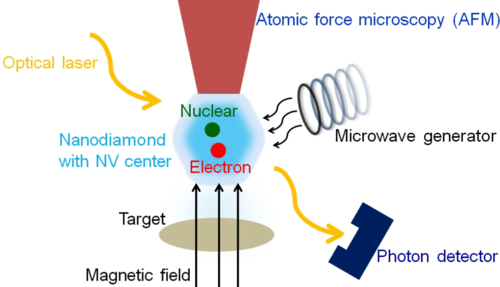
\includegraphics[width=0.45\textwidth]{figures/medium.png}
	}
	\subfigure[A pulse sequence to detect magnetic fields with an electron spin and a nuclear spin in the NV center of diamond.]{
		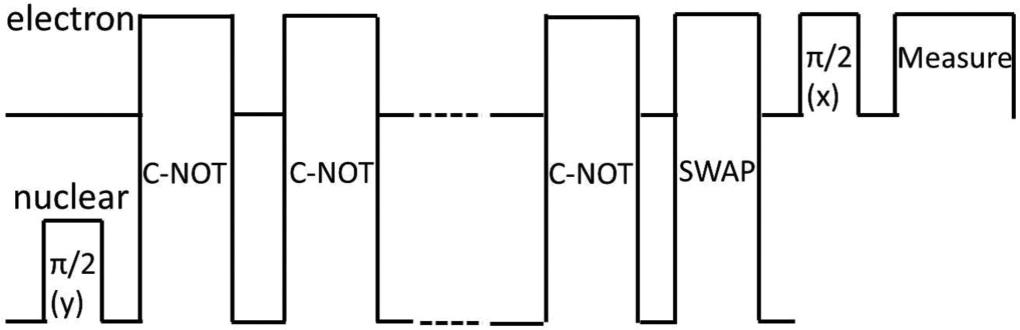
\includegraphics[width=0.45\textwidth]{figures/hybride-nvcenter-magsensor 1.png}
	}
	\caption{The experiment setup and pulse sequence of the magnetic field quantum sensor with NV center defect diamond.}
\end{figure}

\section{Features and Difficulties of Quantum Sensor}
Due to the precision and sensitivity of the quantum sensors, a bright wide futural application in biological science, microelectromechanical systems, experimental physics like photon detectors, called avalanche photodiode, based on detecting entangled photons. With additional cooling process and improvement of quantum senors, it can be used where photomultiplier tube in the field such as medical imaging. However, decoherence and environmental noises constrain the development of quantum sensors, which mainly affects the spatial extensibility of the layout of the sensor's quantum system and temporal sustainability. Decoherence means quantum system loses its interference properties or, in another word, superposition state would vanish and the total system behaves more "classical". A famous example of decoherence is single electron interference experiment describing a single-electron generator emitting a single electron that moves through a two-hole electron barrier then hits on an electron detector. After passing through the two-hole barrier, the single electron could interference with itself to generate an interference pattern on the detector. However, if we try to observe the electron's trajectory during the interference part, the interference pattern will be killed. Actually, when we try to detect the behavior of your quantized electron, some additional probe physical quantities like photons or magnetic fields should be injected into the system. Those kinds of quantities would interact with the particles inside the system or even break the energy spectrum. That will cause decoherence happens. In specific problems, decoherence could also be classified into dephasing and relaxation. Decoherence will lose the superposition information and phase information of the quantum system which will systematically cause information loss. Therefore, decoherence is recognized as the biggest "enemy" of quantum information theory. Although researchers trying to put up new designs of qubit coupled systems to increase the decoherence time in recent years, decoherence analysis still is the most sophisticated and central problem that needs to be solved and it has a long tough way to be that place.

\section{Conclusion}
We briefly introduce the basic concepts of quantum sensing and quantum sensor, from the advantages like high precision and sensitivity to the features and difficulties including the decoherence effect and the tradeoff between decoherence and extensibility. The mechanism of the quantum sensor, qubit, has been introduced covering the definition and coupling between multiply qubit systems. Finally, we conclude a theoretical design of a hybrid quantum magnetic-field sensor with an electron spin and a nuclear spin in NV defect diamond.





\newpage
% \printbibliography
\bibliographystyle{IEEEtran}
\bibliography{references}

\appendix
\section*{Appendix}

\begin{figure}[H]
	\centering
	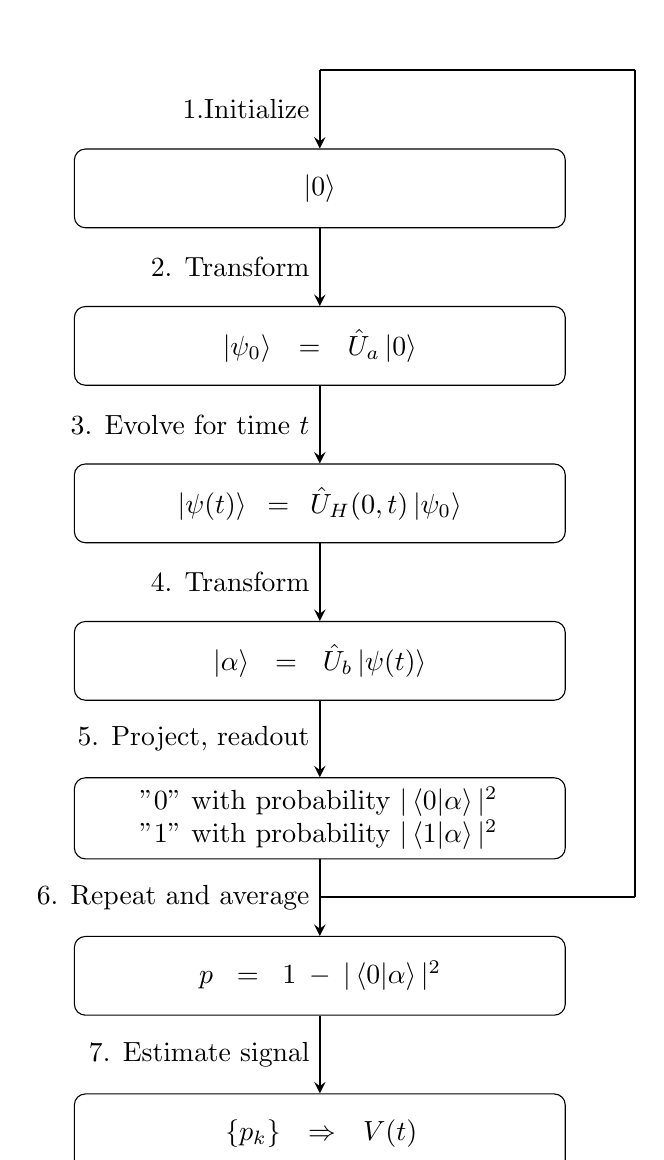
\begin{tikzpicture}[node distance=2cm]
		\centering
		\node (initial) [startstop] {$\ket{0}$};
		\node (transform) [startstop, below of=initial] {$\ket{\psi_0} = \hat{U}_a \ket{0}$};
		\node (evolve) [startstop, below of=transform] {$\ket{\psi(t)} = \hat{U}_H(0,t) \ket{\psi_0}$};
		\node (trans) [startstop, below of=evolve] {$\ket{\alpha} = \hat{U}_b \ket{\psi(t)}$};
		\node (readout) [startstop, below of=trans] {"0" with probability $|\braket{0|\alpha}|^2$ "1" with probability $|\braket{1|\alpha}|^2$};
		\node (repeat) [startstop, below of= readout] {$p=1-|\braket{0|\alpha}|^2$};
		\node (estimate) [startstop, below of=repeat] {$\{p_k\} \Rightarrow V(t)$};
		
		\draw [arrow] (initial) -- node[anchor=east] {2. Transform} (transform);
		\draw [arrow] (transform) -- node[anchor=east] {3. Evolve for time $t$} (evolve);
		\draw [arrow] (evolve) -- node[anchor=east] {4. Transform} (trans);
		\draw [arrow] (trans) -- node[anchor=east] {5. Project, readout} (readout);
		\draw [arrow] (readout) -- node[anchor=east] {6. Repeat and average} (repeat);
		\draw [arrow] (repeat) -- node[anchor=east] {7. Estimate signal} (estimate);
		\draw [line] (0,-9) -- (4,-9);
		\draw [line] (4,-9) -- (4,1.5);
		\draw [line] (4,1.5) -- (0,1.5);
		\draw [arrow] (0,1.5) -- node[anchor=east] {1.Initialize} (initial);
		
		\end{tikzpicture}
		\caption{Basic steps of the quantum sensing process}
\end{figure}

\end{document}